\section{An Example} 

\begin{figure}[t]
\begin{center}
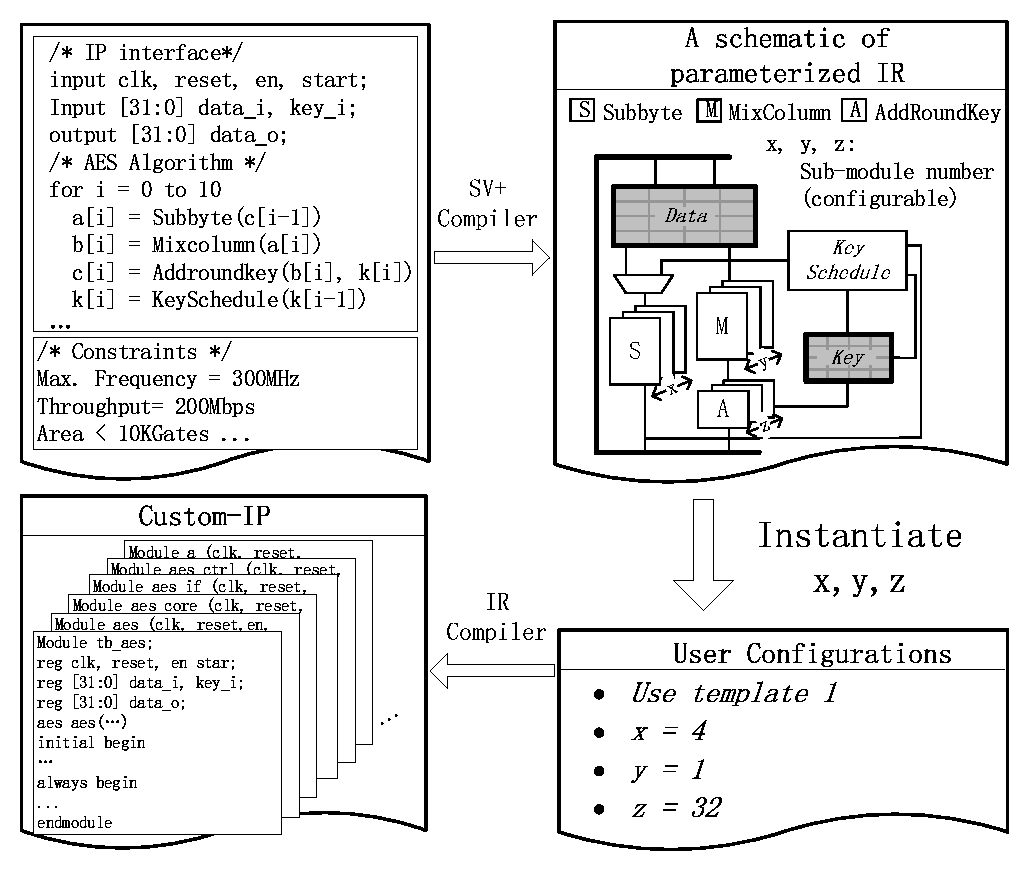
\epsfig{file=example.eps, width=\columnwidth}
\caption{The synthesis of AES IP core}\label{fig-example}
\end{center}
\end{figure}

As an example, Figure \ref{fig-example} illustrates of the synthesis of an AES IP core. 
AES \cite{AES} is a new encryption standard which is widely used in 
both software and hardware designs. 
Different applications call for AES IP cores with different speed, area, and frequency. 
There are four main functions in the AES algorithm: {\tt Subbyte(S)}, 
{\tt Mixcolumn(M)}, {\tt Addroundkey(A)}, and {\tt KeySchedule}. 
All of these functions can be represented by arithmetic transformation modules.   

To automatically generate a specific type of AES core, 
the designer first describes the AES algorithm, the IP interface and constraints in SV+. 
The SV+ code is then preprocessed into a parameterized IR with
five components: {\em Register}, $S$, $M$, $A$, and {\em KeySchedule}. 
Each component corresponds to a function in the AES algorithm, and all of them 
are pre-designed in libraries. 
The template library contains the abstract view of these components, 
such as the interface, timing and area information. 
The preprocessor generates a number of possible templates that implements this algorithm,
and the schematic of one such template (template 1) is shown in the figure.
The number of copies of $S$, $M$ and $A$ are configurable by variable $x$, $y$, and $z$.
The module library contains the detailed hardware implementation of these modules. 
Once instantiated with the user configuration file, a custom AES IP core is automatically generated
by the IR compiler.  

